\documentclass{./../../Latex/handout}
\begin{document}
\thispagestyle{plain}
\myheader{Problem Set 4}
\rhead{Problem Set 4}

\textit{Type up your answers in a Word document and then save it as PDF before uploading them to Canvas. 
}

\begin{enumerate}
\item (2 pts) I regressed wealth (dependent variable) on parents' wealth (independent variable) and found an $R^2=0.64$. What does this mean? Does a high $R^2$ imply that I am identifying the causal impact of parents' wealth on children's wealth? 

\item (1 pt) Consider the following linear regression model:
$$ Y = \beta_0 + \beta_1 X + u $$
Show that $E(u|X)=0$ implies  $E(Y|X) = \beta_0 + \beta_1 X $. 

% Question: Napping
\item (3 pts) A study was conducted to investigate the effects of short naps on memory. The study involved 200 participants who were allowed to nap for either 30 or 60 minutes. After waking up, each participant took a short test on short-term recall. The nap duration for each participant was randomly assigned based on a coin flip. Let $Y_i$ denote the score of the $i$'th participant on the test $(0 ≤ Y_i ≤ 100)$, and let $X_i$ denote the length of time the participant slept before the test ($X_i = $ 30 or 60). Consider the following regression model: $$ Y_i = \beta_0 + \beta_1 X_i + u_i $$ 
\begin{enumerate}
  \item Explain what the term $u_i$ represents. Why might different participants have different values of $u_i$?
  \item Do you think here $E(u_i|X_i) =0$? Why or why not? Will the estimated coefficients be biased or unbiased? 
\item The estimated regression is $ \hat{Y}_i = 55 + 0.17 X_i $. Compute the predicted score for a participant who napped for 30 minutes and for a participant who napped for 60 minutes. Compute the estimated gain/loss in score from a longer nap. 
\end{enumerate}

% Question: R-output
\item (3 pts) 
Output from three regression models is presented below. 
\begin{center}
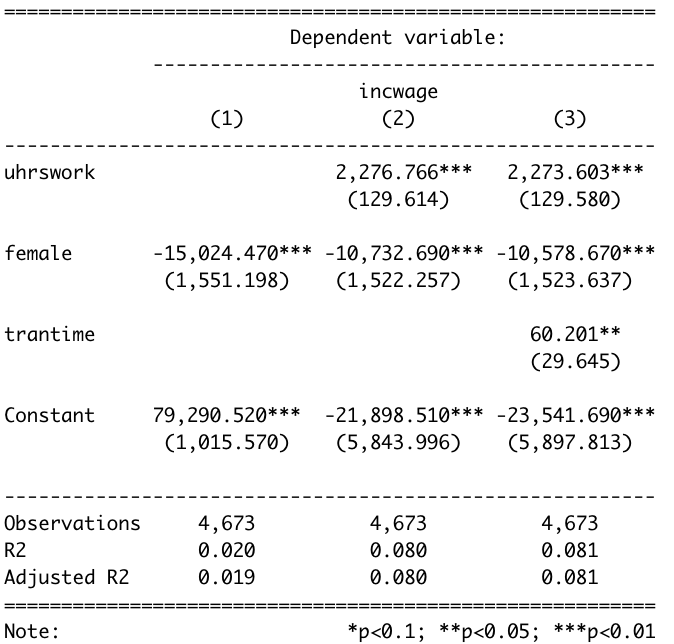
\includegraphics[scale=0.55]{reg.png} 	
\end{center}

The three models are as follows: 
\begin{align*}
	 \text{Model 1:} \quad incwage &=\beta_0 + \beta_1  female + u \\
	 \text{Model 2:} \quad incwage &=\beta_0 + \beta_1  female + \beta_2 uhrswork + u \\
	 \text{Model 3:} \quad incwage &=\beta_0 + \beta_1  female + \beta_2 uhrswork + \beta_3 trantime + u 
\end{align*}

The variables are defined as follows:
\begin{itemize}
  \item \textit{incwage}: annual wage and salary income (in \$)
  \item \textit{female}: indicator variable that takes value 1 for females and 0 for males
  \item \textit{uhrswork}: hours worked each week
  \item \textit{trantime}: transit time to work (in minutes) \\
\end{itemize}

Answer the following questions (0.5 pts each):
\begin{enumerate}
  \item Interpret the coefficient on \textit{female} in Model 1. Is this coefficient statistically significant at a 1\% level of significance?
  \item Interpret the coefficient on \textit{female} from Model 2.
  \item In the second model, we added the variable for hours worked and the coefficient on \textit{female} went down considerably. Given this pattern, do you think women work more or fewer hours than men in our sample? (Note: The coefficient on \textit{uhrswork} is positive.)
  \item Interpret the coefficient on \textit{trantime} in model three. If I wanted to test the null hypothesis that $\beta_3=0$, what would be the associated $t$-value for this test?
\item Find the $p$-value for the $t$-statistic you found in (d).\footnote{You need to refer to the standard normal table or use \texttt{2 * (1 - pnorm(abs(t)))} in R.} What does this $p$-value tell us?
  \item Does the inclusion of \textit{trantime} improve the explanatory power of the regression model for predicting wages? Why or why not?
\end{enumerate}
Pay attention to the units of measurement of each variable while interpreting the coefficients. 

\item (1 pt) Consider the following regression model:
$$ wages_i =\beta_0 +  \beta_1  experience_i + \beta_2 immigrant_i +  \beta_3  experience_i \times immigrant_i + u $$
where $immigrant_i$ is a binary variable that takes the value 1 if an individual is an immigrant and 0 otherwise. $wages_i$ captures earnings and $experience_i$ captures work experience. \\
What is the interpretation of $\beta_3$?  (Hint: Take the expectation of the equation conditional on $immigrant_i=1$ and $immigrant_i=0$.) 
\end{enumerate}
\end{document}